\documentclass{gapd}

\usepackage{lipsum}
\usepackage{natbib}
\usepackage{graphicx}
\usepackage{amsfonts}
\usepackage{amsmath}
\usepackage{subfigure}
\usepackage{booktabs}
\usepackage{multirow}
\usepackage{algorithm}
\usepackage[noend]{algpseudocode}
\bibliographystyle{ieeetr}

\Type{Advanced Machine Learning: Online Learning and Optimization Class Project}
\Title{Online learning on MNIST with multi-expert}

\Author{Letian Chen}{School of Psychological and Cognitive Sciences}

\Abstract{
In this project, I implemented two online learning algorithms (EWA and REWA) and compare them with cross validation choosing multiple candidate algorithms on MNIST dataset. I find that when there is dominant expert (expert that almost right on all data), online learning algorithms will be a little worse than cross validation due to exploration. But when there is no such dominant expert, EWA and REWA will have a much higher performance than cross validation. 
}

% document start
\begin{document}
\maketitle


% ==========Introduction=============
\section{Introduction}
\label{sec:Introduction}
\paragraph{}
	\lettrine{I}{}n the last 5 years, machine learning has been developing at a high speed due to the arising of deep learning. However, the philosophy of deep learning is much different from traditional machine learning methods such as SVM, random forest, decision tree or naive bayes etc. because deep learning is trying to "memorize" the right answer for each example\cite{zhang2016understanding} while most traditional methods are trying to find features or patterns to give the right answer. So it is necessary to combine these two methods to take advantage of both two. It is a straightforward idea to use online learning to choose one of the algorithms' predict (regard each algorithm as an expert and the online learning is to choose one of the experts). With more and more online data and feedback fed in, the online learning algorithm's choice should become more and more smart since it knows which algorithm it should trust. 

\subsection{Task}
\paragraph{}
	I choose a well-known task MNIST. The MNIST database of handwritten digits (See Fig.\ref{fig:MNIST}) has a training set of 60,000 examples, and a test set of 10,000 examples. It is widely used as a simple task for machine learning. Given the $28 \times 28$ pixels, algorithms should classify it into class 0-9 indicating the picture is number 0-9. I also use a simple version of MNIST which contains 1797 examples and each example contains 64 features rather than $28 \times 28$ pixels as a simpler task to compare with the standard MNIST experiment results. 

\begin{figure*}[htb]
	\centering
	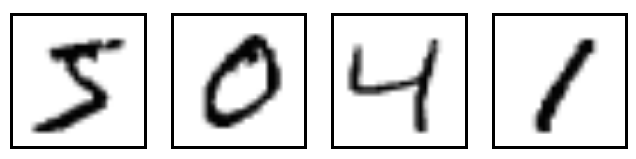
\includegraphics[width=\linewidth / 2]{graph/MNIST}
	\caption{MNIST example}
	\label{fig:MNIST}
\end{figure*}

	
\subsection{Choosed Algorithms}
\paragraph{}
	I choose several classical machine learning methods: 
	\begin{enumerate}
		\item K Nearest Neighbors
		\item Linear SVM
		\item Decision Tree
		\item Random Forest
		\item Multi-layer Perceptron
		\item Ada Boost Classifier
		\item Naive Bayes
		\item Quadratic Discriminant Analysis
	\end{enumerate}
	

\subsection{This project}
\paragraph{}
	In this project, I firstly divide data into 3 parts (training data, cross-validation data and testing data) or 2 parts (training data and testing data) since online learning algorithms don't need cross validation. It is described detailly in Section \ref{sec:Method}. 
\paragraph{}
	Secondly, I apply each algorithms on training data, get its training results and use different methods (cross-validation and online-learning) to do further choice (online-learning choice is actually made in the testing phase) and is described in Section \ref{sec:Method} and the results are shown in Section \ref{sec:Result}. 
\paragraph{}
	Thirdly, I'll show the results on testing data using each method in Section \ref{sec:Result}. 
\paragraph{}
	Finally, I'll analyze the experiment results, discuss it and give some conclusions in Section \ref{sec:discuss_conclusion}. 
% ==========/Introduction=============


% ==========Method=============
\section{Method}
\label{sec:Method}
\paragraph{}
	\lettrine{F}{}irstly to be clear that the methods I talk about here aren't the machine learning algorithms but are cross-validation and online-learning methods. This project is to compare the performance between cross-validation and online-learning methods for the choice after the machine learning algorithms have been trained. 
	
\begin{table}[htb]
\caption{Data dividing for cross validation}
\label{table:data_dividing_cv}
\begin{tabular}{*{3}{c}}
    \toprule 
    \specialrule{0em}{2pt}{2pt}
	Method & CV & Online learning \\
	\specialrule{0em}{2pt}{2pt}
    \midrule
    \multicolumn{1}{l}{Simple MNIST} \\
	\multicolumn{1}{l}{\quad Training} & 1400 & 1597 \\
	\multicolumn{1}{l}{\quad CV} & 197 & 0 \\
	\multicolumn{1}{l}{\quad Test} & 200 & 200 \\
    \multicolumn{1}{l}{Full MNIST} \\
	\multicolumn{1}{l}{\quad Training} & 50000 & 60000 \\
	\multicolumn{1}{l}{\quad CV} & 10000 & 0 \\
	\multicolumn{1}{l}{\quad Test} & 10000 & 10000 \\
    \bottomrule
\end{tabular}
\end{table}
	
\subsection{Cross Validation}
\paragraph{}
	In the cross validation setting, I divide data into 3 parts (training data, cross-validation data and testing data) as shown in Table \ref{table:data_dividing_cv}. Then I train all algorithms using training data. After that I use cross validation (CV) data to choose one of the algorithms: apply all algorithms on cross validation data and choose the algorithm with highest cross validation accuracy. 
	Finally, the algorithm is applied on testing data and get its accuracy on testing data. 

\subsection{Online Learning}
\paragraph{}
	In the online learning setting, I divide data into 2 parts (training data and testing data) as shown in Table \ref{table:data_dividing_cv}. Then I train all algorithms using training data. After that I apply online learning algorithm treating the testing phase as a sequential task and regarding every algorithm as an expert. 
	Finally when the sequential test task is ended, we get its accuracy on testing data. 

\subsubsection{EWA}
\paragraph{}
	The Exponential Weights Algorithm (EWA) is a straightforward method to combine multiple experts by maintaining a weight and every time when given the loss function the weight is exponentially edited. But the averaged prediction may not be integer. So after it I'll take the integer which is nearest to the original prediction as the final prediction. The detail description of algorithm is following (Note that the $\eta \gets \sqrt{\frac{8lnN}{n}} $ is chosen according to the theorem that when $\eta = \sqrt{\frac{8lnN}{n}} $, the worst-case regret of EWA will be at most $\sqrt{\frac12nlnN}$): 

\begin{algorithm}
\caption{Exponential Weights Algorithm}
\label{algo:EWA}
\begin{algorithmic}
\State{set $\eta \gets \sqrt{\frac{8lnN}{n}} $}
\State{set initial weights $w_{0,1},...,w_{0,N} = 1$} 
\For{\texttt{time $t = 1,2,...,n$}}
\State{Receive predictions $f_{t,1} , f_{t,2}, ..., f_{t,N} \in D$ of the experts.}
\State{Predict $p_t = round(\frac{\sum_{i=1}^{N}{w_{t-1,i}f_{t,i}}}{\sum_{i=1}^{N}{w_{t-1,i}}})$}
\State{Receive the loss function $ l_t \in L$ and incur the loss $l_t(p_t)$}
\For{\texttt{$i = 1,2,...,N$}}
	\State{Update $w_{t,i} \gets w_{t-1,i}e^{-\eta l_t(f_{t,i})}$}
  \EndFor
\EndFor
\end{algorithmic}
\end{algorithm}

\subsubsection{REWA}
\paragraph{}

	Randomized Exponential Weights Algorithm (REWA) is only a little different with EWA that it does not choose the "average" predict but to sample a predict of algorithms taking the weight as probability. The detail description of algorithm is listed in Algorithm \ref{algo:REWA} (Note that the $\eta \gets \sqrt{\frac{8lnN}{n}} $ is chosen according to the theorem that when $\eta = \sqrt{\frac{8lnN}{n}} $, the expected regret can be bounded by $\sqrt{\frac12nlnN}$). 

\begin{algorithm}[htb]
\caption{Randomized Exponential Weights Algorithm}
\label{algo:REWA}
\begin{algorithmic}
\State{set $\eta \gets \sqrt{\frac{8lnN}{n}} $}
\State{set initial weights $w_{0,1},...,w_{0,N} = 1$} 
\For{\texttt{time $t = 1,2,...,n$}}
\State{Receive predictions $f_{t,1} , f_{t,2}, ..., f_{t,N} \in D$ of the experts.}
\For{\texttt{$i = 1,2,...,N$}}
	\State{Update $\bar{w}_{t,i} = \frac{w_{t-1,i}}{\sum_{j=0}^{N}{w_{t-1,j}}}$}
\EndFor
\State{Draw $I_t \in {1, 2, . . . , N}$ at random where $Pr[I_t=i]=\bar{w}_{t-1,i}$}
\State{Predict $P_t = f_{t,I_t}$}
\State{Receive the loss function $ l_t \in L$ and incur the loss $l_t(p_t)$}
\For{\texttt{$i = 1,2,...,N$}}
	\State{Update $w_{t,i} \gets w_{t-1,i}e^{-\eta l_t(f_{t,i})}$}
\EndFor
\EndFor
\end{algorithmic}
\end{algorithm}

% ==========/Method=============


% ==========Result=============
\section{Result}
\label{sec:Result}
\paragraph{}
	\lettrine{T}{}he result part is divided into two parts: simple MNIST and full MNIST task. As was said in Section \ref{sec:Introduction}, the simple MNIST datasets contains 1797 examples and each example is an a vector of 64 features. And the full MNIST datasets contains 70000 examples and each example contains $28 \times 28$ pixels. 
	
\subsection{Simple MNIST}
\paragraph{}
	Simple MNIST doesn't have much interesting results since the task is much to easy for some of the algorithms since 3 algorithms can reach an cross validation accuracy of 90\%(See Table \ref{table:simple_MNIST_cv}).
	The cross validation always chooses K Nearest Neighbors, and its test accuracy is 98.5\%. 

\begin{table}[htb]
\caption{Simple MNIST cross validation result}
\label{table:simple_MNIST_cv}
\begin{tabular}{*{2}{c}}
    \toprule 
    \specialrule{0em}{2pt}{2pt}
	 & CV accuracy  \\
	\specialrule{0em}{2pt}{2pt}
    \midrule
    \multicolumn{1}{l}{K Nearest Neighbors} & 96\% \\
	\multicolumn{1}{l}{Linear SVM} & 92\% \\
	\multicolumn{1}{l}{Decision Tree} & 65\% \\
	\multicolumn{1}{l}{Random Forest} & 78\% \\
    \multicolumn{1}{l}{MLP} & 90\% \\
	\multicolumn{1}{l}{Ada Boost} & 28\% \\
	\multicolumn{1}{l}{Naive Bayes} & 80\% \\
	\multicolumn{1}{l}{QDA} & 76\% \\
    \bottomrule
\end{tabular}
\end{table}

	If using EWA and REWA, the result is a little worse than cross validation. The EWA test accuracy is 92\% while the REWA test accuracy is 95.5\%. The reason why online learning algorithm is a little worse than cross validation is that the online learning algorithm needs to explore for some time and during exploring it wastes some of its accuracy. And the final weight of EWA and REWA all almost fall in the nearest neighbors algorithm (because it has greatest accuracy) so the final performance is close to cross validation which chooses nearest neighbors algorithm for every testing data. 

\subsection{Full MNIST}
\paragraph{}
	
	The full MNIST task is much harder than simple MNIST, and no wonder many algorithms' performance decline (see Table \ref{table:full_MNIST_cv}). But the K nearest neighbors, linear SVM and MLP algorithm can still reach CV accuracy over 90\%. So the result will be similar to the simple MNIST since the online learning algorithm will choose K nearest neighbors almost all the time after some exploration (See Figure \ref{fig:weights}). The testing result indicates this is exactly the case: the cross validation chooses nearest neighbors and its accuracy is 96.9\%, the EWA's accuracy is 95.5\% and the REWA's accuracy is 96.6\%. 
	
\begin{figure*}[htb]
\centering
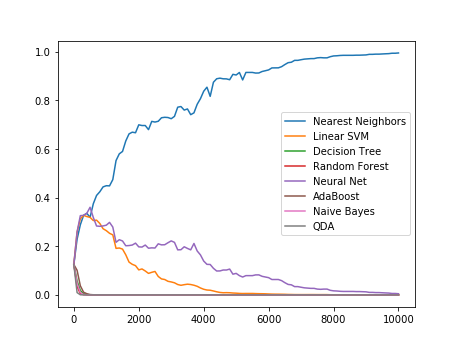
\includegraphics[width=\linewidth / 2]{graph/weights}
\caption{Weights changing during testing}
\label{fig:weights}
\end{figure*}
	
\begin{table}[htb]
\caption{Full MNIST cross validation result}
\label{table:full_MNIST_cv}
\begin{tabular}{*{2}{c}}
    \toprule 
    \specialrule{0em}{2pt}{2pt}
	 & CV accuracy  \\
	\specialrule{0em}{2pt}{2pt}
    \midrule
    \multicolumn{1}{l}{K Nearest Neighbors} & 97.3\% \\
	\multicolumn{1}{l}{Linear SVM} & 94.6\% \\
	\multicolumn{1}{l}{Decision Tree} & 69.4\% \\
	\multicolumn{1}{l}{Random Forest} & 70.4\% \\
    \multicolumn{1}{l}{MLP} & 95.8\% \\
	\multicolumn{1}{l}{Ada Boost} & 75.1\% \\
	\multicolumn{1}{l}{Naive Bayes} & 60.4\% \\
	\multicolumn{1}{l}{QDA} & 10.29\% \\
    \bottomrule
\end{tabular}
\end{table}
	

\subsection{Further results}
\paragraph{}

	Further more, I do some other experiments whose results are interesting. 
	First of all, I decrease the training data of full MNIST. It originally have 60000 training data. Now I reduce the number n's training data to $500 \times (n+1)$, which means that I have 500 training data for number 0 and 5000 training data for number 9. I choose this setup to increase the difficulty to predict some of the data in testing phase since testing data is balanced among all the numbers. Cross validation data is still 1000 examples for each number. So in this setup the cross validation data is very important for some numbers such as 0 and 1. In cross validation method they can not be taken into account since they are cross validation data but the online learning algorithms can. So in this setup, the testing accuracy of cross validation which chooses nearest neighbors (See Table \ref{table:difficult_full_MNIST_cv}) is 96.9\% while the EWA accuracy is 95.5\% and REWA accuracy is 96.6\%. This result is similar to the original test because there is still algorithm whose performance is much better than others and as a result online learning is similar to cross validation except for the exploration. 
	
\begin{table}[htb]
\caption{Difficult Full MNIST cross validation result}
\label{table:difficult_full_MNIST_cv}
\begin{tabular}{*{2}{c}}
    \toprule 
    \specialrule{0em}{2pt}{2pt}
	 & CV accuracy  \\
	\specialrule{0em}{2pt}{2pt}
    \midrule
    \multicolumn{1}{l}{K Nearest Neighbors} & 96.5\% \\
	\multicolumn{1}{l}{Linear SVM} & 93.5\% \\
	\multicolumn{1}{l}{Decision Tree} & 60.3\% \\
	\multicolumn{1}{l}{Random Forest} & 37.5\% \\
    \multicolumn{1}{l}{MLP} & 94.4\% \\
	\multicolumn{1}{l}{Ada Boost} & 67.3\% \\
	\multicolumn{1}{l}{Naive Bayes} & 57.3\% \\
	\multicolumn{1}{l}{QDA} & 17.7\% \\
    \bottomrule
\end{tabular}
\end{table}
	
	Secondly, I rule out some algorithms which have much better performance over others because if so, the online learning algorithm will eventually be identical to cross validation algorithm and it can not take advantage of its dynamic choosing strategy. The cross validation result is no wonder identical to table \ref{table:difficult_full_MNIST_cv} but to rule out K nearest neighbors, linear SVM and MLP algorithms. So the cross validation method will choose AdaBoost and gain test accuracy of 65.5\%. However, the EWA's test accuracy is 69.4\% and the REWA's test accuracy is 71.5\%, both higher than cross validation method. 

% ==========/Result=============


% ==========Discuss and conclusion=============
\section{Discuss and conclusion}
\label{sec:discuss_conclusion}
\paragraph{}
\lettrine{I}{}n the result section, we can see that if the task is easy and some algorithms can get much higher performance than other algorithms, then the online learning algorithm will soon adapt its weight to the only one algorithm and then it is identical to cross validation algorithm. We also see that in most case that REWA algorithm is better than EWA algorithm. That is because the average and round operation is arbitrary and therefore may choose an option that no algorithm chooses (for example, half algorithms choose 2 and the other half choose 5, then the averaging result is 3.5. but either 3 or 4 isn't the algorithms' proposal). On the contrary, the REWA algorithm won't make this kind of mistake. 
\paragraph{}
	In the last part of result section, I show that when the task is hard and there is no algorithm can reach a accuracy over 70\%, both two online learning algorithms are better than cross validation algorithm. Especially, the REWA algorithm is 6 percent higher accurate than cross validation, indicating its good performance when there is no single algorithm that is almost always accurate, the online learning algorithm is much better than cross validation. 
\paragraph{}
	In conclusion, the online learning algorithm's performance is better than cross validation algorithm's when there isn't a dominant expert who is almost always right (because if so, the cross validation will choose this expert and always apply its algorithm, and online learning will gradually give all weights to this expert and finally two kinds of algorithms are identical). Even if there is a dominant expert, the online learning algorithms' accuracy is a little bit lower than cross validation due to the exploration. The other reason why online learning  perform better than cross validation is that cross validation needs some data to do cross validation while online learning algorithms don't need to and can use these data as train data. 
		
% ==========/Discuss and conclusion=============


\section*{Acknowledgements}

Thanks to Teacher Andras Gyorgy and Teacher Assistant Kai Zheng

\section{Reference}
\bibliography{reference}

\end{document}
